\documentclass[12pt,a4paper]{report}
\usepackage[T2A]{fontenc}
\usepackage[utf8]{inputenc}
\usepackage[russian]{babel}
\usepackage[LGRgreek]{mathastext}
\usepackage{graphicx, setspace, multirow, amsmath}
\usepackage[table,xcdraw]{xcolor}
\usepackage{slashbox}

\usepackage[
top = 1.25cm,
bottom = 2.0cm]{geometry}

\makeatletter
\newcommand{\mathleft}{\@fleqntrue\@mathmargin0pt}
\newcommand{\mathcenter}{\@fleqnfalse}
\makeatother

% ========== settings ==========
\newcommand{\strikethroughcolor}{black!50}
\newcommand{\strikethroughwidth}{.25pt}

\newcommand{\strikethroughCrossWidth}{3em}


% ========== styles ==========
\makeatletter
\newcommand{\strikethroughColumnStylePerpendicular}{\let\@markcol@start=\@markcol@start@perpendicular}
\newcommand{\strikethroughColumnStyleDiagonal}{\let\@markcol@start=\@markcol@start@diagonal}
\newcommand{\strikethroughColumnStyleCounterdiagonal}{\let\@markcol@start=\@markcol@start@counterdiagonal}
\newcommand{\strikethroughColumnStyleCross}{\let\@markcol@start=\@markcol@start@cross}

\begin{document}
\begin{titlepage}
	\centering
    % HEADER
	{
        \scshape
        Федеральное государственное автономное образовательное учреждение высшего образования
        \par
        \textbf{«Научно-образовательная корпорация ИТМО»}
        \par
        \vspace*{1cm}
        Факультет Программной Инженерии и Компьютерной Техники
        \par
    }
    % LOGO
    \vspace*{0.6cm}
    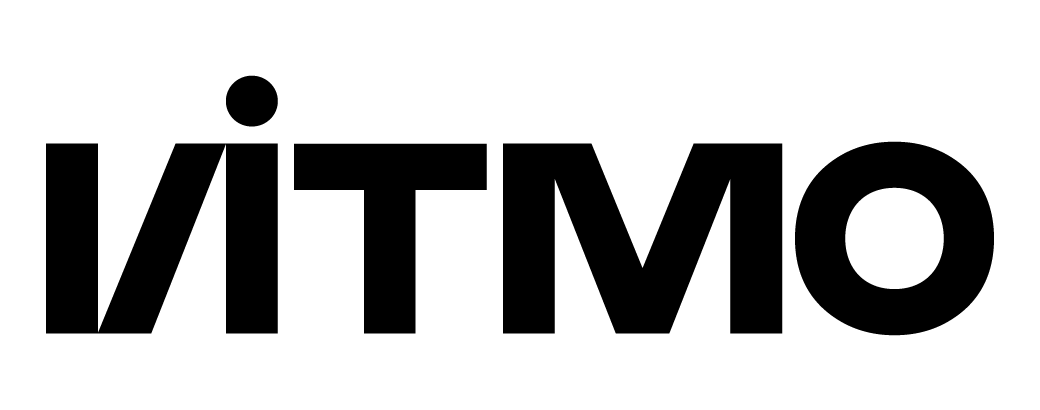
\includegraphics[width=\textwidth]{logo.png}
    % LAB INFO
    {
        \Large
        \textbf{Курсовая работа\\ <<Синтез комбинаторных схем>>\\ Часть №1}
        \par 
        \normalsize
        \vspace*{0.75cm}
        \textbf{Вариант 48}
        \par
    }
    \vfill
    % СREDITS
    \hfill\begin{minipage}{\dimexpr\textwidth-7.8cm}
        \textbf{Выполнил:}\par
        Степанов Арсений Алексеевич\par
        \vspace*{0.15cm}
        \textbf{Группа:}\par
        P3109\par
        \vspace*{0.15cm}
        \textbf{Преподаватель:}\par
        Поляков Владимир Иванович\par
    \end{minipage}
    \vfill
    Санкт-Петербург, \the\year{}г.
\end{titlepage}
\section*{Определение функции}
Функция принимает значение истины, при $2<|x_3x_40-x_5x_1x_2|\leq5$ и безразличное, при $|x_3x_40 - x_5x_1x_2|= 1$.
\section*{Таблица истинности}
\begin{tabular}{|ccccc|c|c|c|c|}
    \hline
    $x_1$ & $x_2$ & $x_3$ & $x_4$ & $x_5$ & $x_3x_40$ & $x_5x_1x_2$ & $|x_3x_40-x_5x_1x_2|$ & $f(x_1\dots x_5)$\\
    \hline
    $0$ & $0$ & $0$ & $0$ & $0$ & $000_2$ & $000_2$ & $0$ & $0$\\
    \hline
    $0$ & $0$ & $0$ & $0$ & $1$ & $000_2$ & $100_2$ & $4$ & $1$\\
    \hline
    $0$ & $0$ & $0$ & $1$ & $0$ & $010_2$ & $000_2$ & $2$ & $0$\\
    \hline
    $0$ & $0$ & $0$ & $1$ & $1$ & $010_2$ & $100_2$ & $2$ & $0$\\
    \hline
    $0$ & $0$ & $1$ & $0$ & $0$ & $100_2$ & $000_2$ & $4$ & $1$\\
    \hline
    $0$ & $0$ & $1$ & $0$ & $1$ & $100_2$ & $100_2$ & $0$ & $0$\\
    \hline
    $0$ & $0$ & $1$ & $1$ & $0$ & $110_2$ & $000_2$ & $6$ & $0$\\
    \hline
    $0$ & $0$ & $1$ & $1$ & $1$ & $110_2$ & $100_2$ & $2$ & $0$\\
    \hline
    $0$ & $1$ & $0$ & $0$ & $0$ & $000_2$ & $001_2$ & $1$ & $d$\\
    \hline
    $0$ & $1$ & $0$ & $0$ & $1$ & $000_2$ & $101_2$ & $5$ & $1$\\
    \hline
    $0$ & $1$ & $0$ & $1$ & $0$ & $010_2$ & $001_2$ & $1$ & $d$\\
    \hline
    $0$ & $1$ & $0$ & $1$ & $1$ & $010_2$ & $101_2$ & $3$ & $1$\\
    \hline
    $0$ & $1$ & $1$ & $0$ & $0$ & $100_2$ & $001_2$ & $3$ & $1$\\
    \hline
    $0$ & $1$ & $1$ & $0$ & $1$ & $100_2$ & $101_2$ & $1$ & $d$\\
    \hline
    $0$ & $1$ & $1$ & $1$ & $0$ & $110_2$ & $001_2$ & $5$ & $1$\\
    \hline
    $0$ & $1$ & $1$ & $1$ & $1$ & $110_2$ & $101_2$ & $1$ & $d$\\
    \hline
    $1$ & $0$ & $0$ & $0$ & $0$ & $000_2$ & $010_2$ & $2$ & $0$\\
    \hline
    $1$ & $0$ & $0$ & $0$ & $1$ & $000_2$ & $110_2$ & $6$ & $0$\\
    \hline
    $1$ & $0$ & $0$ & $1$ & $0$ & $010_2$ & $010_2$ & $0$ & $0$\\
    \hline
    $1$ & $0$ & $0$ & $1$ & $1$ & $010_2$ & $110_2$ & $4$ & $1$\\
    \hline
    $1$ & $0$ & $1$ & $0$ & $0$ & $100_2$ & $010_2$ & $2$ & $0$\\
    \hline
    $1$ & $0$ & $1$ & $0$ & $1$ & $100_2$ & $110_2$ & $2$ & $0$\\
    \hline
    $1$ & $0$ & $1$ & $1$ & $0$ & $110_2$ & $010_2$ & $4$ & $1$\\
    \hline
    $1$ & $0$ & $1$ & $1$ & $1$ & $110_2$ & $110_2$ & $0$ & $0$\\
    \hline
    $1$ & $1$ & $0$ & $0$ & $0$ & $000_2$ & $011_2$ & $3$ & $1$\\
    \hline
    $1$ & $1$ & $0$ & $0$ & $1$ & $000_2$ & $111_2$ & $7$ & $0$\\
    \hline
    $1$ & $1$ & $0$ & $1$ & $0$ & $010_2$ & $011_2$ & $1$ & $d$\\
    \hline
    $1$ & $1$ & $0$ & $1$ & $1$ & $010_2$ & $111_2$ & $5$ & $1$\\
    \hline
    $1$ & $1$ & $1$ & $0$ & $0$ & $100_2$ & $011_2$ & $1$ & $d$\\
    \hline
    $1$ & $1$ & $1$ & $0$ & $1$ & $100_2$ & $111_2$ & $3$ & $1$\\
    \hline
    $1$ & $1$ & $1$ & $1$ & $0$ & $110_2$ & $011_2$ & $3$ & $1$\\
    \hline
    $1$ & $1$ & $1$ & $1$ & $1$ & $110_2$ & $111_2$ & $1$ & $d$\\
    \hline
\end{tabular}
\subsubsection*{КДНФ:}
$f=\overline{x_1}\,\overline{x_2}\,\overline{x_3}\,\overline{x_4}\,x_5\,\vee \,\overline{x_1}\,\overline{x_2}\,x_3\,\overline{x_4}\,\overline{x_5}\,\vee \,\overline{x_1}\,x_2\,\overline{x_3}\,\overline{x_4}\,x_5\,\vee \,\overline{x_1}\,x_2\,\overline{x_3}\,x_4\,x_5\,\vee \,\overline{x_1}\,x_2\,x_3\,\overline{x_4}\,\overline{x_5}\,\vee\vee \,\overline{x_1}\,x_2\,x_3\,x_4\,\overline{x_5}\,\vee \,x_1\,\overline{x_2}\,\overline{x_3}\,x_4\,x_5\,\vee \,x_1\,\overline{x_2}\,x_3\,x_4\,\overline{x_5}\,\vee \,x_1\,x_2\,\overline{x_3}\,\overline{x_4}\,\overline{x_5}\,\vee \,x_1\,x_2\,\overline{x_3}\,x_4\,x_5\,\vee\vee \,x_1\,x_2\,x_3\,\overline{x_4}\,x_5\,\vee \,x_1\,x_2\,x_3\,x_4\,\overline{x_5}$
\subsubsection*{ККНФ:}
$f=(x_1\vee \,x_2\vee \,x_3\vee \,x_4\vee \,x_5)\,\wedge \,(x_1\vee \,x_2\vee \,x_3\vee \,\overline{x_4}\vee \,x_5)\,\wedge \,(x_1\vee \,x_2\vee \,x_3\vee \,\overline{x_4}\vee \,\overline{x_5})\,\wedge\wedge \,(x_1\vee \,x_2\vee \,\overline{x_3}\vee \,x_4\vee \,\overline{x_5})\,\wedge \,(x_1\vee \,x_2\vee \,\overline{x_3}\vee \,\overline{x_4}\vee \,x_5)\,\wedge \,(x_1\vee \,x_2\vee \,\overline{x_3}\vee \,\overline{x_4}\vee \,\overline{x_5})\,\wedge \,(\overline{x_1}\vee\\\vee \,x_2\vee \,x_3\vee \,x_4\vee \,x_5)\,\wedge \,(\overline{x_1}\vee \,x_2\vee \,x_3\vee \,x_4\vee \,\overline{x_5})\,\wedge \,(\overline{x_1}\vee \,x_2\vee \,x_3\vee \,\overline{x_4}\vee \,x_5)\,\wedge \,(\overline{x_1}\vee \,x_2\vee \,\overline{x_3}\vee\vee \,x_4\vee \,x_5)\,\wedge \,(\overline{x_1}\vee \,x_2\vee \,\overline{x_3}\vee \,x_4\vee \,\overline{x_5})\,\wedge \,(\overline{x_1}\vee \,x_2\vee \,\overline{x_3}\vee \,\overline{x_4}\vee \,\overline{x_5})\,\wedge \,(\overline{x_1}\vee \,\overline{x_2}\vee \,x_3\vee \,x_4\vee \,\overline{x_5})\,$
\section*{Минимизация методом Квайна--Мак-Класки}
\subsubsection*{Нахождение максимальных кубов} 
\begin{tabular}{|ccc|}
    \hline
    \multicolumn{3}{|c|}{$K^0(f)$}\\
    \hline
    $1$ & $00001$ & $\vee$\\
    $4$ & $00100$ & $\vee$\\
    $8$ & $01000$ & $\vee$\\
    \hline
    $9$ & $01001$ & $\vee$\\
    $10$ & $01010$ & $\vee$\\
    $12$ & $01100$ & $\vee$\\
    $24$ & $11000$ & $\vee$\\
    \hline
    $11$ & $01011$ & $\vee$\\
    $13$ & $01101$ & $\vee$\\
    $14$ & $01110$ & $\vee$\\
    $19$ & $10011$ & $\vee$\\
    $22$ & $10110$ & $\vee$\\
    $26$ & $11010$ & $\vee$\\
    $28$ & $11100$ & $\vee$\\
    \hline
    $15$ & $01111$ & $\vee$\\
    $27$ & $11011$ & $\vee$\\
    $29$ & $11101$ & $\vee$\\
    $30$ & $11110$ & $\vee$\\
    \hline
    $31$ & $11111$ & $\vee$\\
    \hline
\end{tabular}
\begin{tabular}{|ccc|}
    \hline
    \multicolumn{3}{|c|}{$K^1(f)$}\\
    \hline
    $1-9$ & $0X001$ & \\
    $4-12$ & $0X100$ & \\
    $8-9$ & $0100X$ & $\vee$\\
    $8-10$ & $010X0$ & $\vee$\\
    $8-12$ & $01X00$ & $\vee$\\
    $8-24$ & $X1000$ & $\vee$\\
    \hline
    $9-11$ & $010X1$ & $\vee$\\
    $9-13$ & $01X01$ & $\vee$\\
    $10-11$ & $0101X$ & $\vee$\\
    $10-14$ & $01X10$ & $\vee$\\
    $10-26$ & $X1010$ & $\vee$\\
    $12-13$ & $0110X$ & $\vee$\\
    $12-14$ & $011X0$ & $\vee$\\
    $12-28$ & $X1100$ & $\vee$\\
    $24-26$ & $110X0$ & $\vee$\\
    $24-28$ & $11X00$ & $\vee$\\
    \hline
    $11-15$ & $01X11$ & $\vee$\\
    $11-27$ & $X1011$ & $\vee$\\
    $13-15$ & $011X1$ & $\vee$\\
    $13-29$ & $X1101$ & $\vee$\\
    $14-15$ & $0111X$ & $\vee$\\
    $14-30$ & $X1110$ & $\vee$\\
    $19-27$ & $1X011$ & \\
    $22-30$ & $1X110$ & \\
    $26-27$ & $1101X$ & $\vee$\\
    $26-30$ & $11X10$ & $\vee$\\
    $28-29$ & $1110X$ & $\vee$\\
    $28-30$ & $111X0$ & $\vee$\\
    \hline
    $15-31$ & $X1111$ & $\vee$\\
    $27-31$ & $11X11$ & $\vee$\\
    $29-31$ & $111X1$ & $\vee$\\
    $30-31$ & $1111X$ & $\vee$\\
    \hline
\end{tabular}
\begin{tabular}{|ccc|}
    \hline
    \multicolumn{3}{|c|}{$K^2(f)$}\\
    \hline
    $8-9-10-11$ & $010XX$ & $\vee$\\
    $8-9-12-13$ & $01X0X$ & $\vee$\\
    $8-10-12-14$ & $01XX0$ & $\vee$\\
    $8-10-24-26$ & $X10X0$ & $\vee$\\
    $8-12-24-28$ & $X1X00$ & $\vee$\\
    \hline
    $9-11-13-15$ & $01XX1$ & $\vee$\\
    $10-11-14-15$ & $01X1X$ & $\vee$\\
    $10-11-26-27$ & $X101X$ & $\vee$\\
    $10-14-26-30$ & $X1X10$ & $\vee$\\
    $12-13-14-15$ & $011XX$ & $\vee$\\
    $12-13-28-29$ & $X110X$ & $\vee$\\
    $12-14-28-30$ & $X11X0$ & $\vee$\\
    $24-26-28-30$ & $11XX0$ & $\vee$\\
    \hline
    $11-15-27-31$ & $X1X11$ & $\vee$\\
    $13-15-29-31$ & $X11X1$ & $\vee$\\
    $14-15-30-31$ & $01XX1$ & $\vee$\\
    $26-27-30-31$ & $11X1X$ & $\vee$\\
    $28-29-30-31$ & $111XX$ & $\vee$\\
    \hline
\end{tabular}\\
\begin{tabular}{|ccc|}
    \hline
    \multicolumn{3}{|c|}{$K^3(f)$}\\
    \hline
    $8-9-10-11-12-13-14-15$ & $01XXX$ & $\phantom{\vee}$\\
    $8-10-12-14-24-26-28-30$ & $X1XX0$ & $\phantom{\vee}$\\
    \hline
    $10-11-14-15-26-27-30-31$ & $X1X1X$ & $\phantom{\vee}$\\
    $12-13-14-15-28-29-30-31$ & $X11XX$ & $\phantom{\vee}$\\
    \hline
\end{tabular}
\begin{tabular}{|ccc|}
    \hline
    \multicolumn{3}{|c|}{$K^4(f)$}\\
    \hline
    $\phantom{\vee}$ & $\emptyset$ & $\phantom{\vee}$\\
    \hline
\end{tabular}
\begin{tabular}{|c|}
    \hline
    $Z(f)$\\
    \hline
    $0X001$\\
    $0X100$\\
    $1X011$\\
    $1X110$\\
    $01XXX$\\
    $X1XX0$\\
    $X1X1X$\\
    $X11XX$\\
    \hline
\end{tabular}
\pagebreak
\subsubsection*{Нахождение ядра покрытия}
Построим таблицу импликант:\\
\hfill\break
\begin{tabular}{|c|c|c|c|c|c|c|c|c|c|c|c|c|c|}
    \hline
    \multicolumn{2}{|c|}{}                                    & \multicolumn{12}{|c|}{Существенные вершины}                                                                                                                                                                                                                                                                                                                                                                                                                                                                                                                                                                                                                                                                                                                                                                                                                                                                                                                                                                            \\ \cline{3-14} 
    \multicolumn{2}{|c|}{}                                    & \cellcolor[HTML]{9AFF99}\begin{tabular}[c]{@{}l@{}}0\\ 0\\ 0\\ 0\\ 1\end{tabular} & \cellcolor[HTML]{9AFF99}\begin{tabular}[c]{@{}l@{}}0\\ 0\\ 1\\ 0\\ 0\end{tabular} & \cellcolor[HTML]{9AFF99}\begin{tabular}[c]{@{}l@{}}0\\ 1\\ 0\\ 0\\ 1\end{tabular} & \begin{tabular}[c]{@{}l@{}}0\\ 1\\ 0\\ 1\\ 1\end{tabular} & \cellcolor[HTML]{9AFF99}\begin{tabular}[c]{@{}l@{}}0\\ 1\\ 1\\ 0\\ 0\end{tabular} & \cellcolor[HTML]{9AFF99}\begin{tabular}[c]{@{}l@{}}0\\ 1\\ 1\\ 1\\ 0\end{tabular} & \cellcolor[HTML]{9AFF99}\begin{tabular}[c]{@{}l@{}}1\\ 0\\ 0\\ 1\\ 1\end{tabular} & \cellcolor[HTML]{9AFF99}\begin{tabular}[c]{@{}l@{}}1\\ 0\\ 1\\ 1\\ 0\end{tabular} & \cellcolor[HTML]{9AFF99}\begin{tabular}[c]{@{}l@{}}1\\ 1\\ 0\\ 0\\ 0\end{tabular} & \cellcolor[HTML]{9AFF99}\begin{tabular}[c]{@{}l@{}}1\\ 1\\ 0\\ 1\\ 1\end{tabular} & \cellcolor[HTML]{9AFF99}\begin{tabular}[c]{@{}l@{}}1\\ 1\\ 1\\ 0\\ 1\end{tabular} & \cellcolor[HTML]{9AFF99}\begin{tabular}[c]{@{}l@{}}1\\ 1\\ 1\\ 1\\ 0\end{tabular} \\ \cline{3-14} 
    \multicolumn{2}{|c|}{\multirow{-3}{*}{Максимальные кубы}} & \cellcolor[HTML]{9AFF99}1                                                         & \cellcolor[HTML]{9AFF99}4                                                         & \cellcolor[HTML]{9AFF99}9                                                         & 11                                                        & \cellcolor[HTML]{9AFF99}12                                                        & \cellcolor[HTML]{9AFF99}14                                                        & \cellcolor[HTML]{9AFF99}19                                                        & \cellcolor[HTML]{9AFF99}22                                                        & \cellcolor[HTML]{9AFF99}24                                                        & \cellcolor[HTML]{9AFF99}27                                                        & \cellcolor[HTML]{9AFF99}29                                                        & \cellcolor[HTML]{9AFF99}30                                                        \\ \hline
    \rowcolor[HTML]{FFFFC7} 
    \cellcolor[HTML]{FFCCC9}A & \cellcolor[HTML]{FFCCC9}0X001 & X                                                                                 &                                                                                   & X                                                                                 & \cellcolor[HTML]{FFCCC9}                                  &                                                                                   &                                                                                   &                                                                                   &                                                                                   &                                                                                   &                                                                                   &                                                                                   &                                                                                   \\ \hline
    \rowcolor[HTML]{FFFFC7} 
    \cellcolor[HTML]{FFCCC9}B & \cellcolor[HTML]{FFCCC9}0X100 &                                                                                   & X                                                                                 &                                                                                   & \cellcolor[HTML]{FFCCC9}                                  & X                                                                                 &                                                                                   &                                                                                   &                                                                                   &                                                                                   &                                                                                   &                                                                                   &                                                                                   \\ \hline
    \rowcolor[HTML]{FFFFC7} 
    \cellcolor[HTML]{FFCCC9}C & \cellcolor[HTML]{FFCCC9}1X011 &                                                                                   &                                                                                   &                                                                                   & \cellcolor[HTML]{FFCCC9}                                  &                                                                                   &                                                                                   & X                                                                                 &                                                                                   &                                                                                   & X                                                                                 &                                                                                   &                                                                                   \\ \hline
    \rowcolor[HTML]{FFFFC7} 
    \cellcolor[HTML]{FFCCC9}D & \cellcolor[HTML]{FFCCC9}1X110 &                                                                                   &                                                                                   &                                                                                   & \cellcolor[HTML]{FFCCC9}                                  &                                                                                   &                                                                                   &                                                                                   & X                                                                                 &                                                                                   &                                                                                   &                                                                                   & X                                                                                 \\ \hline
    E                         & 01XXX                         & \cellcolor[HTML]{9AFF99}                                                          & \cellcolor[HTML]{9AFF99}                                                          & \cellcolor[HTML]{9AFF99}X                                                         & X                                                         & \cellcolor[HTML]{9AFF99}X                                                         & \cellcolor[HTML]{9AFF99}X                                                         & \cellcolor[HTML]{9AFF99}                                                          & \cellcolor[HTML]{9AFF99}                                                          & \cellcolor[HTML]{9AFF99}                                                          & \cellcolor[HTML]{9AFF99}                                                          & \cellcolor[HTML]{9AFF99}                                                          & \cellcolor[HTML]{9AFF99}                                                          \\ \hline
    \rowcolor[HTML]{FFFFC7} 
    \cellcolor[HTML]{FFCCC9}F & \cellcolor[HTML]{FFCCC9}X1XX0 &                                                                                   &                                                                                   &                                                                                   & \cellcolor[HTML]{FFCCC9}                                  & X                                                                                 & X                                                                                 &                                                                                   &                                                                                   & X                                                                                 &                                                                                   &                                                                                   & X                                                                                 \\ \hline
    \rowcolor[HTML]{FFFFC7} 
    \cellcolor[HTML]{FFCCC9}G & \cellcolor[HTML]{FFCCC9}X11XX &                                                                                   &                                                                                   &                                                                                   & \cellcolor[HTML]{FFCCC9}                                  & X                                                                                 & X                                                                                 &                                                                                   &                                                                                   &                                                                                   &                                                                                   & X                                                                                 & X                                                                                 \\ \hline
    H                         & X1X1X                         & \cellcolor[HTML]{9AFF99}                                                          & \cellcolor[HTML]{9AFF99}                                                          & \cellcolor[HTML]{9AFF99}                                                          & X                                                         & \cellcolor[HTML]{9AFF99}                                                          & \cellcolor[HTML]{9AFF99}X                                                         & \cellcolor[HTML]{9AFF99}                                                          & \cellcolor[HTML]{9AFF99}                                                          & \cellcolor[HTML]{9AFF99}                                                          & \cellcolor[HTML]{9AFF99}X                                                         & \cellcolor[HTML]{9AFF99}                                                          & \cellcolor[HTML]{9AFF99}X                                                         \\ \hline
\end{tabular}\\
\hfill\break
\mathleft
По таблице определяем ядро покрытия:\\
\begin{equation*}
    \mbox{T=}
    \begin{cases}
        0X001\\
        0X100\\
        X1XX0\\
        X11XX\\
        1X011\\
        1X110\\
    \end{cases}
\end{equation*}
\subsubsection*{Нахождение минимального покрытия}
Воспользуемся методом Петрика и запишем выражение определяющее условие покрытия всех вершин:\\
$Y=E\vee H$\\
Следовательно получается два возможных покрытия: $C_1=T\vee E$ и $C_2=T\vee H$\\
\begin{equation*}
    C_1=
    \begin{cases}
        0X001\\
        0X100\\
        X1XX0\\
        X11XX\\
        1X011\\
        1X110\\
        01XXX\\
    \end{cases}
    C_2=
    \begin{cases}
        0X001\\
        0X100\\
        X1XX0\\
        X11XX\\
        1X011\\
        1X110\\
        X1X1X\\
    \end{cases}
\end{equation*}
$S_1^a=22$, $S_1^b=29$\\
$S_2^a=22$, $S_2^b=29$\\
\hfill\break
Цены покрытий совпадают, значит они оба могут выступать в роли минимального покрытия.\\
\hfill\break
\hfill\break
Пускай $C_{min}=C_1$\\
\begin{equation*}
    C_{min}=
    \begin{cases}
        0X001\\
        0X100\\
        X1XX0\\
        X11XX\\
        1X011\\
        1X110\\
        01XXX\\
    \end{cases}
\end{equation*}
$S_{min}^a=22$, $S_{min}^b=29$\\
\hfill\break
МДНФ минимального покрытия:\\
$C_{min}=\overline{x_1}\,\overline{x_3}\,\overline{x_4}\,x_5\vee\overline{x_1}\,x_3\,\overline{x_4}\,\overline{x_5}\vee x_2\,\overline{x_5}\vee x_2\,x_3\vee x_1\,\overline{x_3}\,x_4\,x_5\vee x_1\,x_3\,x_4\,\overline{x_5}\vee \overline{x_1}\,x_2$
\section*{Минимизация методом карт Карно}
\subsubsection*{МДНФ}
\includegraphics[width=13cm]{karno1.png}
\begin{equation*}
    C_{min}=
    \begin{cases}
        0X001\\
        0X100\\
        X1XX0\\
        X11XX\\
        1X011\\
        1X110\\
        01XXX\\
    \end{cases}
\end{equation*}
$S_{min}^a=22$, $S_{min}^b=29$\\
\hfill\break
$C_{min}=\overline{x_1}\,\overline{x_3}\,\overline{x_4}\,x_5\vee\overline{x_1}\,x_3\,\overline{x_4}\,\overline{x_5}\vee x_2\,\overline{x_5}\vee x_2\,x_3\vee x_1\,\overline{x_3}\,x_4\,x_5\vee x_1\,x_3\,x_4\,\overline{x_5}\vee \overline{x_1}\,x_2$\\
\pagebreak
\subsubsection*{МКНФ}
\includegraphics[width=13cm]{karno2.png}
\begin{equation*}
    C_{min}=
    \begin{cases}
        00X1X\\
        X00X0\\
        X01X1\\
        1X001\\
        10X0X\\
    \end{cases}
\end{equation*}
$S_{min}^a=16$, $S_{min}^b=21$\\
\hfill\break
$C_{min}=(x_1\vee x_2\vee \overline{x_4})(x_2\vee x_3\vee x_5)(x_2\vee\overline{x_3}\vee\overline{x_5})(\overline{x_1}\vee x_3\vee x_4\vee \overline{x_5})(\overline{x_1}\vee x_2\vee x_4)$
\section*{Преобразование минимальных форм}
\subsubsection*{Факторизация и декомпозиция МДНФ}
\begin{tabular}{lc}
$f=\overline{x_1}\,\overline{x_3}\,\overline{x_4}\,x_5\vee\overline{x_1}\,x_3\,\overline{x_4}\,\overline{x_5}\vee x_2\,\overline{x_5}\vee x_2\,x_3\vee x_1\,\overline{x_3}\,x_4\,x_5\vee x_1\,x_3\,x_4\,\overline{x_5}\vee \overline{x_1}\,x_2$ & $S_Q=29, \tau=2$\\
$f=x_2\,(\overline{x_1}\vee  x_3\vee\overline{x_5})\vee (\overline{x_1}\,\overline{x_4}\vee x_1\,x_4)(x_3\overline{x_5}\vee\overline{x_3}x_5)$ & $S_Q=21, \tau=4$\\ 
$\varphi=\overline{x_3}x_5$, $\overline{\varphi}=x_3\vee\overline{x_5}$\\
$f=x_2(\overline{\varphi}\vee\overline{x_1})\vee(\overline{x_1}\,\overline{x_4}\vee x_1\,x_4)(x_3\overline{x_5}\vee\varphi)$ & $S_Q=21, \tau=5$\\
В данном случае декомпозиция нецелесообразна & \\
$f=x_2\,(\overline{x_1}\vee  x_3\vee\overline{x_5})\vee (\overline{x_1}\,\overline{x_4}\vee x_1\,x_4)(x_3\overline{x_5}\vee\overline{x_3}x_5)$ & $S_Q=21, \tau=4$\\ 
\end{tabular}
\subsubsection*{Факторизация и декомпозиция МКНФ}
\begin{tabular}{lc}
$f=(x_1\vee x_2\vee \overline{x_4})(x_2\vee x_3\vee x_5)(x_2\vee\overline{x_3}\vee\overline{x_5})(\overline{x_1}\vee x_3\vee x_4\vee \overline{x_5})(\overline{x_1}\vee x_2\vee x_4)$ & $S_Q=21$, $\tau=2$\\
$f=(x_2\vee (x_1 \vee \overline{x_4})(x_3\vee x_5)(\overline{x_3}\vee \overline{x_5}))(\overline{x_1} \vee x_3 \vee x_4 \vee \overline{x_5})(\overline{x_1} \vee x_2 \vee x_4)$ & $S_Q=21$, $\tau=4$\\
Декомпозиция в данном случае невозможна & \\
$f=(x_2\vee (x_1 \vee \overline{x_4})(x_3\vee x_5)(\overline{x_3}\vee \overline{x_5}))(\overline{x_1} \vee x_3 \vee x_4 \vee \overline{x_5})(\overline{x_1} \vee x_2 \vee x_4)$ & $S_Q=21$, $\tau=4$\\
\end{tabular}
\newpage
\section*{Синтез комбинаторных схем}
Анализировать схемы будем при следующих значениях аргументов:\\
$f(0, 0, 0, 0, 0) = 0$\\
$f(0, 0, 0, 0, 1) = 1$\\
\subsubsection*{Булев базис}
$f=(x_2\vee (x_1 \vee \overline{x_4})(x_3\vee x_5)(\overline{x_3}\vee \overline{x_5}))(\overline{x_1} \vee x_3 \vee x_4 \vee \overline{x_5})(\overline{x_1} \vee x_2 \vee x_4)$\\ $S_Q=21$, $\tau=4$\\
\hfill\break
\includegraphics[width=10cm]{schema1.png}\\
%Схема по упрощённой МКНФ:\\
%$f=(x_2\vee (x_1 \vee \overline{x_4})(x_3\vee x_5)(\overline{x_3}\vee \overline{x_5}))(\overline{x_1} \vee x_3 \vee x_4 \vee \overline{x_5})(\overline{x_1} \vee x_2 \vee x_4)$\\ $S_Q=21$, $\tau=4$\\
%\includegraphics[width=10cm]{schema2.png}\\
\subsubsection*{Сокращённый булев базис (И-НЕ)}
$f=\overline{\overline{x_2\overline{\varphi x_1}}\,\overline{\overline{\overline{\overline{x_1}\,\overline{x_4}}\,\overline{x_1 x_4}}\,\overline{\overline{x_3\overline{x_5}}\,\overline{\varphi}}}}$, $\varphi=\overline{x_3}x_5$\\
$S_Q=30, \tau=8$\\
\includegraphics[width=17cm]{schema3.png}
\newpage
\subsubsection*{Универсальный базис (И-НЕ, 2 входа)}
$f=\overline{\overline{x_2\overline{x_1\overline{\overline{\overline{x_3}\,x_5}}}}\,\overline{\overline{\overline{\overline{x_1}\,\overline{x_4}}\,\overline{x_1x_4}}\,\overline{\overline{x_3\overline{x_5}}\,\overline{\overline{x_3}x_5}}}}$\\
$S_Q=24, \tau=5$\\
\includegraphics[width=15cm]{schema4.png}
\end{document}

